\section{Sprint 1}
Tal y como se ha definido en la sección \ref{sec:planificacion-inicial}, el primer sprint se centra en la base de nuestra aplicación web, desarrollando la estructura inicial del servidor, gestión de usuarios y subida y descarga sencilla de archivos.
Para ello, se han elegido las historias de usuario relacionadas con el objetivo de este sprint y se han desarrollado definiendo sub-historias de usuario si fueran necesarias, criterios de aceptación y las tareas necesarias para su implementación.

Las historias de usuario se han seleccionado de manera aproximada, puesto que al ser el primer sprint no tenemos una velocidad de equipo definida. Existe la posibilidad de que algunas historias de usuario no se completen en este sprint o de que se completen más de las previstas, por lo que se ha dejado un margen de maniobra para que el equipo pueda adaptarse a la realidad del desarrollo.

Cuando se termine el sprint, se calculará la velocidad del equipo la cual se utilizará para planificar los siguientes sprints, de manera que se pueda ajustar la cantidad de historias de usuario a desarrollar en cada uno de ellos.

Una vez definidas todas las tareas que se van a realizar en este sprint, se ha realizado un diagrama de Gantt para planificar el tiempo que se va a dedicar a cada una de ellas, teniendo en cuenta que el sprint tiene una duración de dos semanas, y se dará un orden de prioridad a las tareas que se consideren más importantes para llegar a el objetivo del sprint.

\subsection{Historias de usuario}
En esta sección se detallan las historias de usuario y técnicas que se han elegido para este sprint. Se va a hacer una breve descripción de cada una de ellas, así como los criterios de aceptación y las tareas necesarias para su implementación. Si fuera necesario, se definirán sub-historias de usuario para facilitar su desarrollo.

Las seleccionadas son las siguientes:
\begin{itemize}
    \item HU05: Inicio de sesión - 5 PH
    \item HU06: Cerrar sesión - 2 PH
    \item HU13: Crear cuentas - 8 PH
    \item HT03 API REST en Rust - 13 PH
    \item HT05: Autenticación JWT - 5 PH
    \item HT08: Base de datos - 8 PH
    \item HT18.1: Binario - 2 PH
    \item HT19: Dockerización - 3 PH
    \item HT20.1: Documentación del proyecto en GitHub - 5 PH
    \item HT20.2: Documentación de la API REST con OpenAPI - 5 PH
\end{itemize}

Estas historias de usuario y técnicas suman un total de 56 puntos de historia (PH). Es importante destacar que la estimación en puntos de historia representa la complejidad relativa de cada historia, mientras que las tareas de desarrollo se estiman en horas de trabajo efectivo.

La descomposición en tareas de desarrollo de las historias de usuario se pueden encontrar en el apéndice \ref{appendix:sprint1-backlog}.

El total de horas estimadas para todas las tareas de desarrollo del Sprint 1 es de 56 horas, distribuidas de la siguiente manera:

\begin{itemize}
    \item HU05 (Inicio de sesión): 7 horas
    \item HU06 (Cerrar sesión): 2 horas  
    \item HU13 (Crear cuentas): 8 horas
    \item HT03 (API REST en Rust): 13 horas
    \item HT05 (Autenticación JWT): 5 horas
    \item HT08 (Base de datos): 7 horas
    \item HT18.1 (Binario): 2 horas
    \item HT19 (Dockerización): 3 horas
    \item HT20.1 (Documentación GitHub): 4 horas
    \item HT20.2 (Documentación OpenAPI): 5 horas
\end{itemize}

Esta estimación se ajusta perfectamente a la capacidad del sprint de 2 semanas con 4 horas diarias de dedicación (14 días × 4 horas = 56 horas totales).

Se puede ver que hay historias de usuario con los mismos puntos de historia o parecidos pero con diferente número de horas estimadas. Esto es normal, ya que los puntos de historia representan la complejidad relativa y no el tiempo exacto de desarrollo. Por ejemplo, una historia de usuario puede ser más compleja pero requerir menos tiempo si se reutilizan componentes existentes o se aprovechan bibliotecas ya implementadas.

\subsection{Diagrama de Gantt}
Dada las estimaciones de las tareas, se han considerado el siguiente orden de prioridad de tareas en un diagrama de Gantt:
\begin{figure}[H]
    \begin{center}
        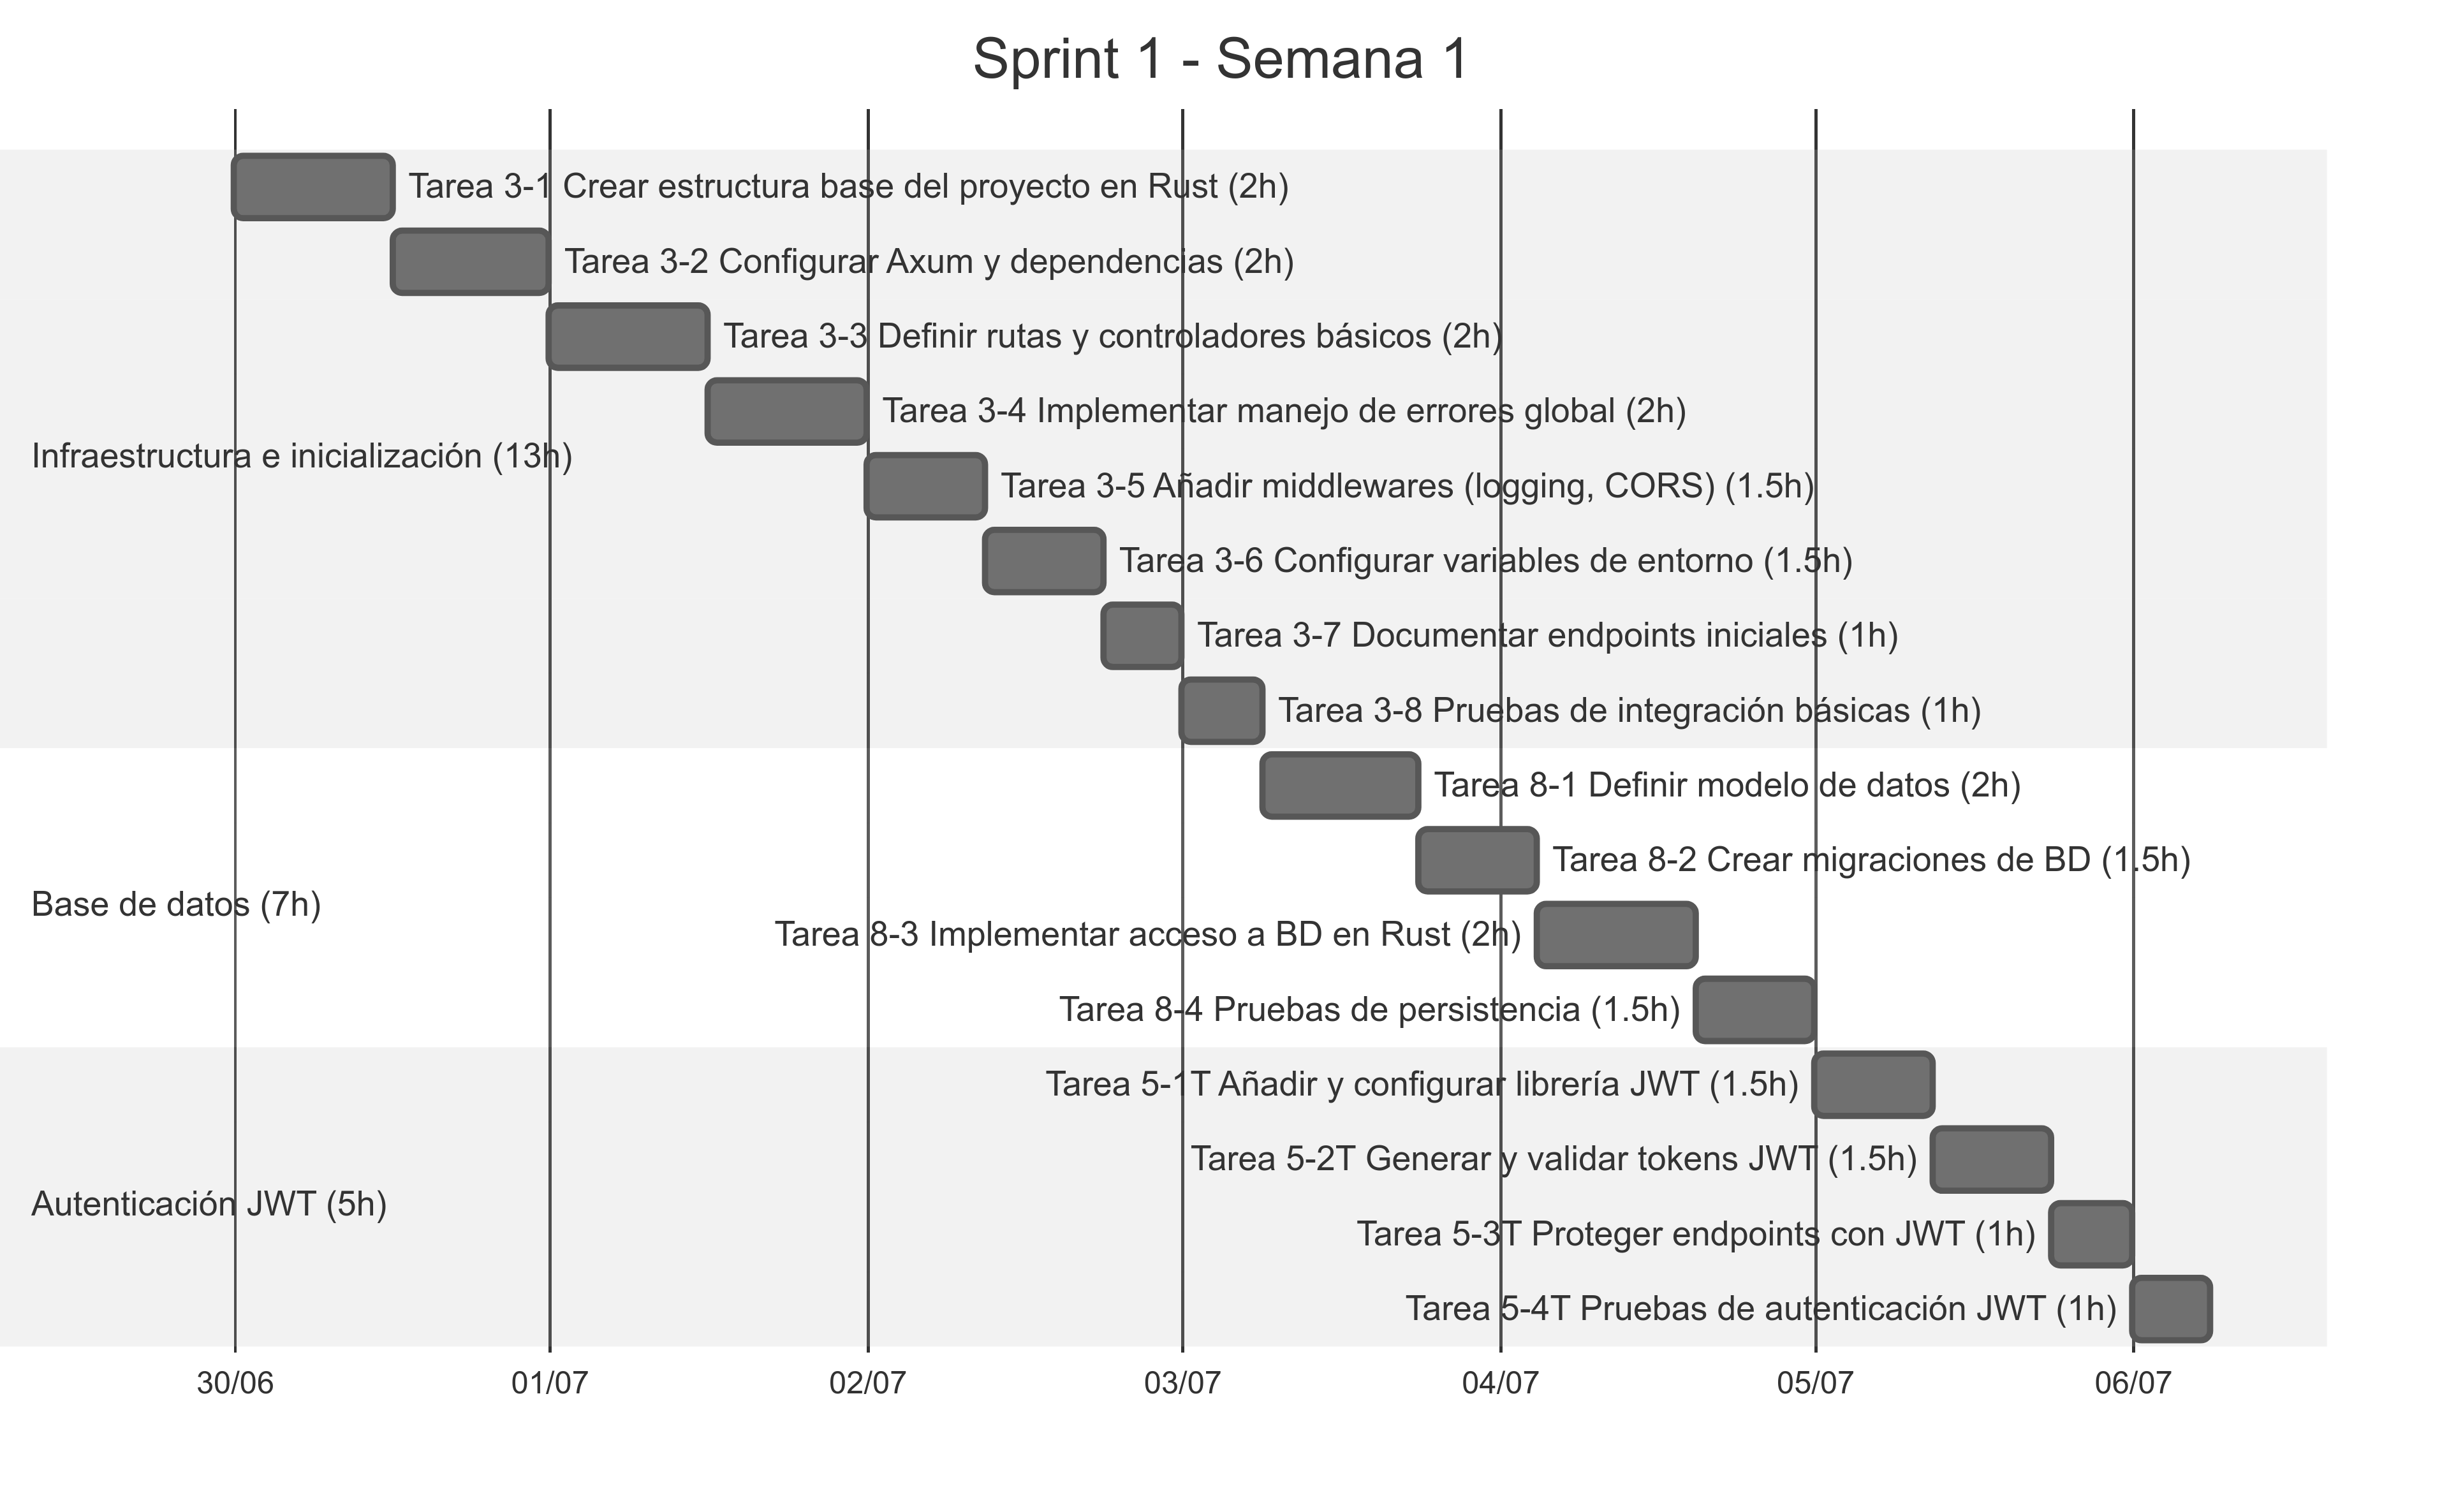
\includegraphics[width=0.8\textwidth]{assets/sprint1/sprint1-week1.png}
    \end{center}
    \caption{Diagrama de Gantt de las tareas de la primera semana del sprint 1}\label{fig:sprint1-week1}
\end{figure}

\begin{figure}[H]
    \begin{center}
        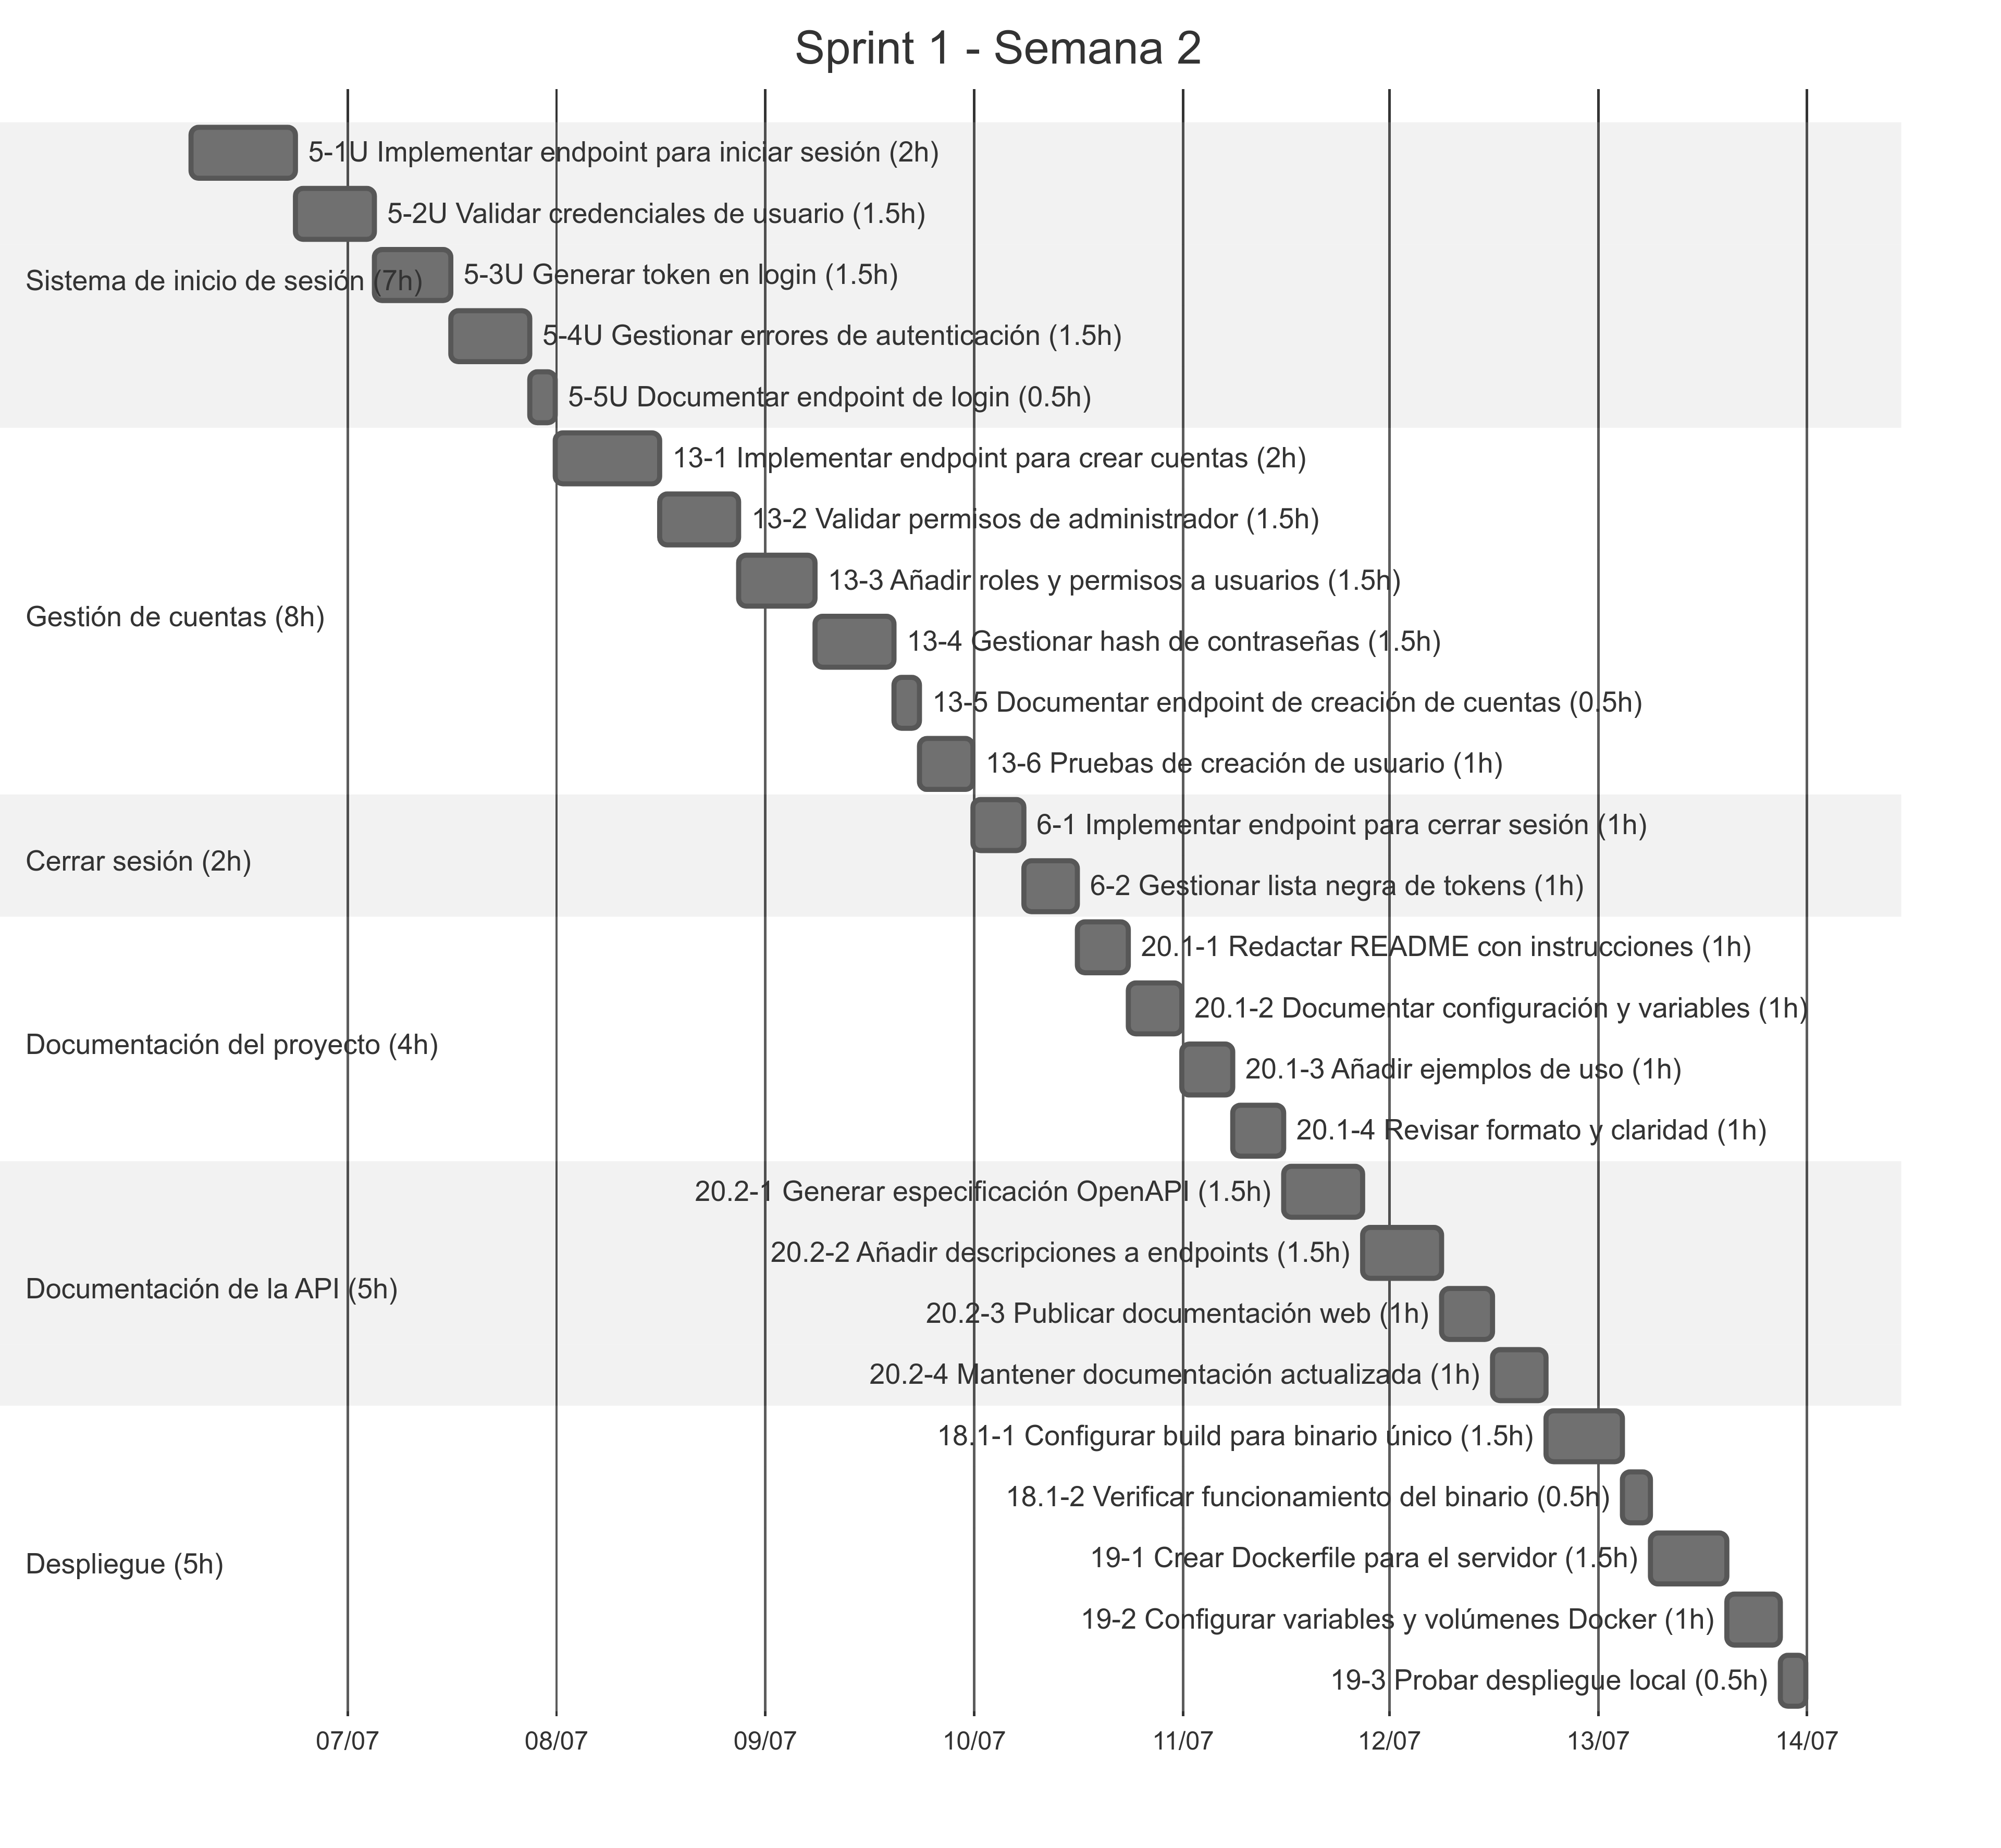
\includegraphics[width=0.8\textwidth]{assets/sprint1/sprint1-week2.png}
    \end{center}
    \caption{Diagrama de Gantt de las tareas de la segunda semana del sprint 1}\label{fig:sprint1-week2}
\end{figure}

Se ha seguido un orden lógico, en el que primero inicializaremos toda la capa de interfaz, en este caso nuestra API, junto con todas las dependencias que nos harán falta a la hora de documentar, errores no genéricos, variables de entorno, pruebas...

Después, se implementará el diseño de la base de datos. Una vez tenemos esta base, se implementarán las primeras funcionalidades, que van a ser la del inicio de sesión seguro, seguido de la gestión de cuentas. Para finalizar el sprint, se documentará todo al completo.

Para finalizar, configuraremos todo lo necesario para poder desplegar el servidor.

\subsection{Diseño detallado e implementación}

\paragraph{Acceso a datos}
\subparagraph{}
Se ha optado por usar el \acrshort{orm} \textbf{Diesel} para el acceso a datos, ya que es uno de los más populares y robustos en el ecosistema de Rust. Diesel proporciona una interfaz segura y eficiente para interactuar con bases de datos SQL, lo que facilita la creación y gestión de esquemas, así como la ejecución de consultas.

Diesel nos proporciona un sistema de migraciones que nos permite versionar y gestionar los cambios en la estructura de la base de datos de manera controlada, generando esquemas que podemos utilizar a la hora de utilizar los métodos que nos proporciona el ORM. De esta manera, tendremos consultas seguras y tipadas.
Esto nos da una especial seguridad a la hora de hacer un desarrollo ágil, ya que podemos iterar rápidamente sobre el modelo de datos y asegurarnos de que los cambios se reflejan correctamente en la base de datos y en nuestro código, ya que hasta que no se solucionen los problemas de compilación provenientes de los cambios en la infraestructura, no se podrá seguir avanzando.

\paragraph{Implementación de Arquitectura Limpia}
\subparagraph{}

Tal y como se ha descrito en apartados anteriores, se ha seguido una arquitectura limpia siguiendo el paradigma de programación \acrshort{cqrs}.

Para ello, se ha aprovechado el sistema de \textit{tipos genéricos} que ofrece Rust.

Los tipos genéricos en Rust permiten escribir código que puede funcionar con múltiples tipos de datos sin necesidad de duplicar el código. Se definen utilizando parámetros de tipo, que son identificadores que se reemplazan por tipos concretos cuando se utiliza el código genérico.

En una arquitectura limpia, los tipos genéricos facilitan la creación de componentes reutilizables e independientes de la implementación concreta. Por ejemplo, se puede definir una interfaz (trait en Rust) para un repositorio de datos y luego implementar diferentes repositorios (e.g., uno para una base de datos y otro para un archivo) que implementen ese trait. Los tipos genéricos permiten que las capas superiores de la aplicación interactúen con el repositorio a través del trait, sin necesidad de conocer la implementación concreta. Esto facilita la inyección de dependencias, donde se puede pasar una implementación concreta del repositorio a la capa superior en tiempo de ejecución.

Los traits en Rust definen un conjunto de métodos que un tipo debe implementar para ser considerado como una instancia de ese trait, se podría considerar que son las ``interfaces'' de Rust. Los traits se pueden usar con tipos genéricos para restringir los tipos que se pueden usar con una función o estructura genérica. Por ejemplo, se puede definir una función genérica que solo funcione con tipos que implementen el trait `Display`.

De esta manera, definimos los traits que nos van a hacer falta en el dominio y cuando queremos usarlo en alguna función, simplemente le pasamos el tipo genérico que está definido en el dominio.
A la hora de inicializar nuestra aplicación es cuando vamos a instanciar los tipos concretos que implementan esos traits que vamos a usar, los cuales se van a inyectar en donde haga falta, por lo general en un estado global de la aplicación, el cual es accesible desde cualquier hilo de ejecución.

Esto se puede ver en el siguiente ejemplo, donde definimos un trait que representa un repositorio de usuarios y luego implementamos el repositorio que accederá a la base de datos mediante el ORM \textbf{Diesel}:

\begin{lstlisting}[language=Rust, caption={Trait de repositorio de usuarios}, label={lst:trait-repository}]
// src/lib/users/domain/user_repository.rs
use std::future::Future;

use crate::users::domain::{user::NewUser, User};

pub trait UserRepository: Clone + Send + Sync + 'static {
    fn get_by_username(
        &self,
        username: String,
    ) -> impl Future<Output = Result<Option<User>, UserRepositoryError>> + Send;
    fn create_user(&self, user: NewUser) -> impl Future<Output = Result<User, UserRepositoryError>> + Send;
}

#[derive(Debug, thiserror::Error)]
pub enum UserRepositoryError {
    #[error("User already exists")]
    UserAlreadyExists,
    #[error("Unexpected error")]
    InternalServerError,
}
\end{lstlisting}
Hemos definido un trait que será usado para acceder de alguna manera que nuestra capa de aplicación no va a saber. Además, se definen errores de dominio, los cuales no tienen nada que ver con cualquier error que pueda ocurrir al acceder a los datos en la base de datos o el sistema que se esté usando.

Además, el trait especifica que su implementación debe también implementar Clone, Send y Sync, asegurando que se pueda utilizar de manera segura entre hilos. Esto es importante para que nuestro repositorio pueda ser usado en un entorno asíncrono y concurrente.

\begin{lstlisting}[language=Rust, caption={Implementación del repositorio de usuarios}, label={lst:impl-repository}]
// src/lib/users/infrastructure/diesel_user_repository.rs
#[derive(Clone)]
pub struct DieselUserRepository {
    pool: Arc<Pool<ConnectionManager<PgConnection>>>,
}

impl DieselUserRepository {
    pub fn new(connection: Arc<Pool<ConnectionManager<PgConnection>>>) -> Self {
        DieselUserRepository { pool: connection }
    }
}

impl UserRepository for DieselUserRepository {
    async fn create_user(&self, new_user: NewUser) -> Result<User, UserRepositoryError> {
        // Implementación de la creación de usuario usando diesel
    }

    async fn get_by_username(
        &self,
        user_username: String,
    ) -> Result<Option<User>, UserRepositoryError> {
        // Implementación de la obtención de usuario por nombre de usuario usando diesel
    }
}
\end{lstlisting}

Aquí podemos ver una implementación del trait que hemos definido anteriormente, en este caso para acceder a una base de datos PostgreSQL mediante el ORM \textbf{Diesel}. Esta implementación es la que se inyectará en el estado global de nuestra aplicación cuando se inicialice.
En este caso, el repositorio implementa Send, Sync y Clone derivándolo de Clone, pues todas sus propiedades las implementan también haciendo que el repositorio lo implemente por ende.

El repositorio usará una pool de conexiones, pues al ser usado por varios hilos, necesitamos que cada hilo tenga su propia conexión a la base de datos para evitar bloqueos y problemas de concurrencia.

Una vez tenemos el trait y su implementación, tan solo nos va a quedar inyectar el repositorio en el estado global y utilizar el estado en nuestra capa de aplicación:
\begin{lstlisting}[language=Rust, caption={Inyección del repositorio en el estado global y uso en el comando para crear un usuario}, label={lst:inject-repository}]
// src/bin/server/main.rs
#[tokio::main]
async fn main() -> anyhow::Result<()> {
    dotenvy::dotenv().ok();


    let connection_pool = Arc::new(establish_connection());

    let user_repository = DieselUserRepository::new(connection_pool);

    let server = HttpServer::new(user_repository).await?;

    server.run().await
}

// src/lib/users/interface/http/routes.rs
pub async fn create_user<UR: UserRepository>(
    State(state): State<AppState<UR>>,
    ValidatedJson(body): ValidatedJson<CreateUserCommand>,
) -> Result<(StatusCode, Json<ApiResponseBody<CreateUserResult>>), ApiError> {
    match create_user_command_handler(body, state.user_repository.as_ref()).await {
        Ok(user) => Ok((
            StatusCode::CREATED,
            ApiResponseBody::new(user).into(),
        )),
        Err(err) => match err {
            UserRepositoryError::UserAlreadyExists => Err(ApiError::ConflictError(err.to_string())),
            UserRepositoryError::InternalServerError => Err(ApiError::InternalServerError(err.to_string())),
        },
    }
}

// src/lib/users/application/commands/create_user.rs
pub async fn create_user_command_handler<UR: UserRepository>(
    mut command: CreateUserCommand,
    user_repository: &UR,
) -> Result<CreateUserResult, UserRepositoryError> {

    if user_repository.get_by_username(command.username.clone()).await?.is_some() {
        return Err(UserRepositoryError::UserAlreadyExists);
    }

    let salt = SaltString::generate(&mut OsRng);

    let argon2 = Argon2::default();

    command.password = argon2
        .hash_password(command.password.as_bytes(), &salt)
        .map_err(|_| UserRepositoryError::InternalServerError)?
        .to_string();

    Ok(user_repository.create_user(command.into()).await?.into())
}
\end{lstlisting}

Cuando definimos el estado global que va a extraer nuestro endpoint mediante el extractor que nos proporciona Axum, lo definimos con un tipo genérico \textit{UR}, el cual especificamos que va a implementar el trait \textit{UserRepository}. Es decir, sabemos los métodos que nos ofrece y las propiedades que tiene que tener, pero en la capa de aplicación no tenemos que conocer cómo se está implementando, solamente cómo se usa.

Otra buena práctica que podemos observar en el código es utilizar errores de dominio. De esta manera, abstraemos la capa de aplicación de cualquier tipo de error que pueda ocurrir en la capa de infraestructura y solamente en la capa de interfaz, que es la que presenta los datos al usuario, asociamos cada error de dominio al error correspondiente de interfaz.

Así, si quisiéramos cambiar cómo accedemos a los datos, tan solo tendríamos que crear o modificar la implementación que realizamos en la capa de infraestructura.

El siguiente diagrama muestra cómo se relacionan las diferentes capas de la arquitectura limpia que hemos implementado:
\begin{figure}[H]
    \begin{center}
        \includegraphics[width=0.95\textwidth]{assets/sprint1/diagrama-arquitectura-limpia.png}
    \end{center}
    \caption{Diagrama del diseño arquitectónico detallado de nuestra implementación.}\label{fig:diagrama-arquitectura-limpia-sprint1}
\end{figure}

Tal como se ha definido en la arquitectura software, la capa de interfaz accede a la capa de aplicación pero no viceversa. Para hacer uso de la capa de infraestructura, la capa de aplicación utiliza una abstracción de dominio que utiliza siempre objetos de dominio, la cual después la infraestructura implementa y se inicializa en el estado global de la aplicación.

\paragraph{Documentación de la API REST}
\subparagraph{}

Para documentar todos los endpoints de la API REST, se ha utilizado la especificación OpenAPI. Esta especificación permite describir de manera estructurada los endpoints, parámetros, tipos de datos y respuestas de la API.

Esta documentación se genera automáticamente mediante la librería \textbf{utoipa}, que se integra con Axum para generar la documentación a partir de los atributos y tipos definidos en el código. 
Esto asegura que la documentación esté siempre actualizada y refleje fielmente el estado actual de la API, por lo que cada vez que definamos un nuevo endpoint o modifiquemos uno existente, la documentación se actualizará automáticamente.

Además, se ha configurado otra librería compatible con utoipa \textbf{utoipa-swagger-ui}, que permite servir la documentación generada como una página web interactiva, lo que facilita a los desarrolladores y usuarios explorar y probar los endpoints de la API, mostrando ejemplos de peticiones, respuestas, errores y los esquemas usados en las peticiones y respuestas.
Además, nos permite probar los endpoints directamente desde la interfaz.

\paragraph{Pruebas unitarias y de integración}
\subparagraph{}

Para garantizar la calidad del código y el correcto funcionamiento de la aplicación, se han implementado pruebas unitarias y de integración utilizando la librería \textbf{tokio} para pruebas asíncronas y un \textbf{servicio oneshot} para simular el servidor HTTP.
El servicio oneshot no es más que un servidor HTTP con unas rutas definidas al igual que nuestra API, solo que es de un solo uso para realizar pruebas, ya que solamente deja simular una sola petición y respuesta, lo que es suficiente para nuestras pruebas unitarias.

En este punto es donde entra en juego una de las ventajas de utilizar una arquitectura limpia y CQRS.
Al separar la lógica de negocio de la infraestructura, podemos probar los comandos y consultas de manera aislada, sin necesidad de depender de la implementación concreta del repositorio o de la base de datos. Esto nos permite escribir pruebas más rápidas y enfocadas en la lógica de negocio.

Además, nos da la ventaja de poder \gls{mockear} los repositorios y otros componentes de infraestructura, lo que facilita la simulación de diferentes escenarios y errores en las pruebas.

Así, tendríamos la siguiente estructura en la carpeta de tests:

\dirtree{%
.1 tests.
.2 tests.rs.
.2 users.
.3 application.
.4 commands.
.5 test\_create\_user.rs.
.5 test\_login.rs.
.4 queries.
.5 test\_get\_all\_users.rs.
.5 test\_get\_user.rs.
.3 domain.
.4 auth.rs.
.4 roles.rs.
.4 user\_repository.rs.
.4 user.rs.
.3 infrastructure.
.4 test\_jwt\_token\_service.rs.
.4 test\_mappers.rs.
.4 test\_models.rs.
.4 test\_repository.rs.
.3 integration.
.4 test\_user\_endpoints.rs.
.3 mocks.rs.
.2 utils.
.3 functions.rs.
}

Como se puede ver, hemos separado las pruebas en diferentes carpetas según su tipo: pruebas de dominio, de infraestructura, de aplicación y de integración.
Se han abarcado todos los casos de uso definidos en las historias de usuario, asegurando que cada funcionalidad se prueba de manera aislada y también en conjunto con el resto del sistema.

Para ejecutar todos los tests, es tan sencillo como ejecutar el comando $cargo\ test$ en la raíz del proyecto, lo que ejecutará todas las pruebas definidas en la carpeta \texttt{tests} y mostrará los resultados en la consola.

\paragraph{Despliegue}
\subparagraph{}

Todos los pasos necesarios para el despliegue se han definido en el README del proyecto, donde se explica cómo construir el binario, cómo crear la imagen Docker y cómo ejecutar el servidor en un contenedor Docker, o directamente del binario compilado.

Nuestra aplicación depende de una base de datos PostgreSQL (de momento) y se ha generado un archivo docker compose para facilitar el despliegue de la aplicación junto con la base de datos. Este archivo define los servicios necesarios, incluyendo el servidor y la base de datos, y permite iniciar todo el entorno con un solo comando.

Si bien se puede utilizar docker compose para levantar el entorno de desarrollo, también se puede ejecutar el servidor directamente desde el binario generado, definiendo en las variables de entorno los parámetros necesarios para la base de datos, sin necesidad de usar Docker.
